\documentclass[14pt,aspectratio=1610]{beamer}

\usepackage[brazil]{babel}
\usepackage[utf8]{inputenc}
%\UseRawInputEncoding
\usepackage[T1]{fontenc}
%\usepackage{Sweave}
\usepackage{animate}
\usepackage{amsbsy}
\usepackage{amsfonts}
\usepackage{amsmath}
\usepackage{amssymb}
\usepackage{amsthm}
\usepackage[toc,page,title,titletoc]{appendix}
%\usepackage[fixlanguage]{babelbib}
%\usepackage[pdftex]{color}
\usepackage{dsfont}
\usepackage{esvect}
\usepackage[labelfont=bf]{caption}
\usepackage{subcaption}
\usepackage{float}
\usepackage[Glenn]{fncychap}%Sonny %Conny %Lenny %Glenn %Renje %Bjarne %Bjornstrup
%\usepackage{geometry, calc, color, setspace}%
%\geometry{a4paper, headsep=1.0cm, footskip=1cm, lmargin=3cm, rmargin=2cm, tmargin=3cm, bmargin=2cm}
\usepackage{graphicx}
\usepackage{indentfirst}%Para indentar os parágrafos automáticamente
\usepackage{lipsum}
\usepackage{longtable}
\usepackage{mathtools}
\usepackage{listings}%Inserir codigo do R no latex
\usepackage{multirow}
\usepackage{multicol}
\usepackage{csquotes}
\usepackage[style = abnt,
			%style = bwl-FU,
			maxcitenames = 2,
			terseinits = true,
			natbib = true, 
			maxbibnames = 99]{biblatex}
\addbibresource{Referencias/Referencias.bib}
\usepackage[figuresright]{rotating}
\usepackage{spalign}
%\usepackage{pgfpages}
\usepackage{pgfplots}
\pgfplotsset{compat=1.18}
\usepackage{tikz}
\usepackage{color, colortbl}
\usepackage{ragged2e}%para justificar o texto dentro de algum ambiente
\definecolor{Gray}{gray}{0.9}
\definecolor{LightCyan}{rgb}{0.88,1,1}
\definecolor{Lightblue}{RGB}{50, 149, 168}
%\usepackage{grffile}

\usepackage[all]{xy}



\usetheme{Madrid}
\usecolortheme[RGB={193,0,0}]{structure}

%\setbeamertemplate{footline}[frame number]
%\setbeamertemplate{footline}[text line]{%
%  \parbox{\linewidth}{\vspace*{-8pt}\hfill\date{}\hfill\insertshortauthor\hfill\insertpagenumber}}
\beamertemplatenavigationsymbolsempty
\renewcommand{\vec}[1]{\mbox{\boldmath$#1$}}
\newtheorem{Teorema}{Teorema}
\newtheorem{Proposicao}{Proposição}
\newtheorem{Definicao}{Definição}
\newtheorem{Corolario}{Corolário}
\newtheorem{Demonstracao}{Demonstração}
\newcommand{\bx}{\ensuremath{\bar{x}}}
\newcommand{\Ho}{\ensuremath{H_{0}}}
\newcommand{\Hi}{\ensuremath{H_{1}}}
\everymath{\displaystyle}

\apptocmd{\frame}{}{\justifying}{} % Allow optional arguments after frame.

\title{Iniciação à Estatística}
\author{Prof. Fernando de Souza Bastos \texorpdfstring{\\ fernando.bastos@ufv.br}{}}
\institute{Departamento de Estatística \texorpdfstring{\\ Universidade Federal de Viçosa}{}\texorpdfstring{\\ Campus UFV - Viçosa}{}}
\date{}
\newcommand\mytext{Aula 3}
\newcommand\mytextt{Fernando de Souza Bastos}
\newcommand\mytexttt{\url{https://ufvest.github.io/}}

\makeatletter
\setbeamertemplate{footline}
{
  \leavevmode%
  \hbox{%
  \begin{beamercolorbox}[wd=.3\paperwidth,ht=2.25ex,dp=1ex,center]{author in head/foot}%
    \usebeamerfont{author in head/foot}\mytext
  \end{beamercolorbox}%
  \begin{beamercolorbox}[wd=.3\paperwidth,ht=2.25ex,dp=1ex,center]{title in head/foot}%
    \usebeamerfont{title in head/foot}\mytextt
  \end{beamercolorbox}%
  \begin{beamercolorbox}[wd=.35\paperwidth,ht=2.25ex,dp=1ex,right]{site in head/foot}%
    \usebeamerfont{site in head/foot}\mytexttt\hspace*{2em}
    \insertframenumber{} / \inserttotalframenumber\hspace*{2ex} 
  \end{beamercolorbox}}%
  \vskip0pt%
}
\makeatother

\providecommand{\arcsin}{} \renewcommand{\arcsin}{\hspace{2pt}\textrm{arcsen}}
\providecommand{\sin}{} \renewcommand{\sin}{\hspace{2pt}\textrm{sen}}
%\newtheorem{Teorema}{Teorema}
%\newtheorem{Proposicao}{Proposição}
%\newtheorem{Definicao}{Definição}
%\newtheorem{Corolario}{Corolário}
%\newtheorem{Demonstracao}{Demonstração}

\titlegraphic{\hspace*{8cm}\href{https://fsbmat-ufv.github.io/}{
\includegraphics[width=2cm]{figs/mylogo.png}}
}


\usepackage{hyperref,bookmark}
\hypersetup{
  colorlinks=true,
  linkcolor=blue,
  citecolor=red,
  filecolor=blue,
  urlcolor=blue,
}

% Layout da pagina
\hypersetup{pdfpagelayout=SinglePage}
\begin{document}
%\Sconcordance{concordance:Aula15.tex:Aula15.Rnw:%
1 339 1}


\frame{\titlepage}

\begin{frame}{}
\frametitle{\bf Sumário}
\tableofcontents
\end{frame}

\section{Medidas de Dispersão}
\begin{frame}{}
\frametitle{}
\begin{block}{}
\justifying
O resumo de um conjunto de dados por uma única medida representativa de posição
central esconde toda a informação sobre a variabilidade do conjunto de observações.
Por exemplo, suponhamos que cinco grupos de alunos submeteram-se a um
teste, obtendo-se as seguintes notas:
\begin{itemize}
\item Grupo A (Variável $X$): 3,4,5,6,7
\item Grupo B (Variável $Y$): 1,3,5,7,9
\item Grupo C (Variável $Z$): 5,5,5,5,5
\item Grupo D (Variável $W$): 3,5,5,7
\item Grupo E (Variável $V$): 3,5,5,6,6
\end{itemize}
\end{block}
\end{frame}

\begin{frame}{}
\frametitle{}
\begin{block}{}
\justifying
Vemos que $\bar{x}=\bar{y}=\bar{z}=\bar{w}=\bar{v}=5$. A identificação de cada uma destas séries por sua
média (5, em todos os casos) nada informa sobre suas diferentes variabilidades. Notamos, então, a conveniência de serem criadas medidas que sumarizem a variabilidade de um conjunto de observações e que nos permita, por exemplo, comparar conjuntos diferentes de valores, como os dados acima, segundo algum critério estabelecido.
\end{block}
\end{frame}

%\begin{frame}{}
%\frametitle{}
%\begin{block}{}
%\justifying
%Um critério freqüentemente usado para tal fim é aquele que mede a dispersão dos
%dados em torno de sua média, e duas medidas são as mais usadas: desvio médio e variância.
%O princípio básico é analisar os desvios das observações em relação à média dessas
%observações.
%\end{block}
%\end{frame}

\begin{frame}{}
\frametitle{}
\begin{block}{}
\justifying
Um critério frequentemente usado para tal fim é aquele que mede a dispersão dos dados em torno de sua média. Duas medidas são as mais usadas: desvio médio e variância.
\begin{align*}
Dm(X) &=\displaystyle \dfrac{{\displaystyle \sum_{i=1}^{n}|x_{i}-\bar{x}|}}{n}&
Var(X)&=\displaystyle \dfrac{{\displaystyle \sum_{i=1}^{n}(x_{i}-\bar{x})^{2}}}{n}
\end{align*}
O princípio básico é analisar os desvios das observações em relação à média dessas observações. Desvio é interpretado como o afastamento de uma observação em relação a uma determinada medida de posição.
\end{block}
\end{frame}

\begin{frame}{}
    \frametitle{Variância Amostral}
    \begin{block}{}
    \justifying
    \begin{equation*}
	S^2(X) = \dfrac{{SQD_X }}{{n - 1}} = \dfrac{{\sum\limits_{i = 1}^n {\left( {X_i  - \bar X} \right)^2 } }}{{n - 1}} = \dfrac{{\sum\limits_{i = 1}^n {X_i^2  - \dfrac{{\left( {\sum\limits_{i = 1}^n {X_i } } \right)^2 }}{n}} }}{{n - 1}}  = \dfrac{\sum\limits_{i = 1}^n {X_i^2  - n \bar{X}^2}}{n-1}
	\end{equation*}
    \end{block}
    \pause
    \begin{block}{}
    Medidas foram tomadas de 3 grupos, os resultados foram:
    	\begin{itemize}
		\item Grupo 1 (em Kg): 1,3,5,7,9
		\item Grupo 2 (em metros): 1.8,3.8,5.8,7.8,9.8 
		\item Grupo 3 (em R\$): 1002,1004,1006,1008,1010
	\end{itemize}
	Calcule a variância destes 3 grupos!
    \end{block}
\end{frame}

\begin{frame}{}
\frametitle{}
\begin{block}{}
\justifying
Sendo a variância uma medida de dimensão igual ao quadrado da dimensão dos dados (por exemplo, se os dados são expressos em $cm,$ a variância será expressa 
em $cm^{2}$), ela pode causar problemas de interpretação. Costuma-se usar, então, o desvio padrão, que é definido como a raiz quadrada positiva da variância.
\begin{equation}
dp(X)=S(X)=\sqrt{Var(X)}
\end{equation}
Ambas as medidas de dispersão ($Dm$ e $dp$) indicam em média qual será o ``erro'' (desvio) cometido ao tentar substituir cada observação pela medida resumo do conjunto de dados (no caso, a média). Resolvido, portanto, o problema da unidade de medida.
\end{block}
\end{frame}

\begin{frame}{}
\frametitle{Coeficiente de Variação}
\begin{block}{}
\justifying
\begin{equation}
CV(X)=\dfrac{dp(X)}{\bar{X}}\cdot 100 = \dfrac{S(X)}{\bar{X}}\cdot 100
\end{equation}
Mesmo o DP pode induzir à conclusões errôneas com relação à variabilidade. Suponha dois conjuntos de dados 
$D_{1}=\{10,20,30\}$ e $D_{2}=\{10000,10010,10020\}.$ Note que nestes casos $\bar{x}_{1}=20, dp(x)=10, 
\bar{x}_{2}=10010$ e $dp(x_{2})=10.$ Porém, em termos percentuais, o primeiro conjunto de dados é mais 
heterogênio.
\end{block}
\pause
\begin{block}{}
\justifying
\noindent \textbf{Obs.}: O C.V. é utilizado para avaliar qual o percentual da média que o desvio-padrão representa. Isso é chamado de homogeneidade. Na situação em que as amostras possuem a mesma média, a conclusão pode ser feita a partir da comparação de suas variâncias. Para amostras com médias diferentes, aquela que apresentar menor CV, é a mais homogênea.
\end{block}
\end{frame}

\begin{frame}{}
    \frametitle{Erro Padrão da Média}
    \begin{block}{}
    \begin{equation*}
	S(\overline{X}) = \sqrt{ \dfrac{S^2(X)}{n} }
	\end{equation*}
	
	\noindent \textbf{Obs.}: É uma medida utilizada para avaliar a precisão da média. 
    \end{block}
    \pause
    \begin{block}{Exemplo}
    Considere duas amostras de tamanhos $n=6$, em que $S^{2}_{A}
= 5,6$ e $S^{2}_{B}= 28.$ Temos que:

\begin{table}[H]
    \centering
    \begin{tabular}{cc}
    $S(\bar{X_{A}})=\sqrt{\dfrac{5,6}{6}}=0,966;$     &  
    $S(\bar{X_{B}})=\sqrt{\dfrac{28}{6}}=2,1602$
    \end{tabular}
\end{table}
e, portanto, a amostra $A$ forneceu uma estimativa de média associada à uma maior precisão. 
    \end{block}
\end{frame}

\begin{frame}{}
\frametitle{Erro Padrão da Média}
    \begin{block}{}
    Notem que o erro padrão da média é:
\begin{itemize}
    \item Inversamente proporcional ao tamanho da amostra;
    \item Diretamente proporcional à variância da amostra.
\end{itemize}
    \end{block}
\end{frame}

\begin{frame}{Amplitude Total}
\begin{block}{}
\justifying
A amplitude total (AT) é dada pela diferença entre o maior e o menor valor de uma amostra ou de um conjunto de dados. Se $X_1, X_2, X_3, \cdots , X_n$ é uma amostra de valores da variável $X,$ então:

$$AT_X = X_{(n)} - X_{(1)}$$

Recorde que a notação $X_{(i)}$ indica estatísticas de ordem da amostra, isto é: $X_{(1)} \leq X_{(2)} \leq X_{(3)} \leq \cdots \leq X_{(n)}.$ Portanto, a amplitude total indica que o desvio entre duas observações quaisquer é no máximo igual a AT.
\end{block}
\end{frame}

\section{Associação entre Variáveis Quantitativas}
\begin{frame}[fragile]{}
\frametitle{Coeficiente de Correlação Amostral}
\vspace{-0.5cm}
\begin{tabular}{cl}  
        \begin{tabular}{c}
          \parbox{0.5\linewidth}{
          \begin{table}[h!]
  \caption{Anos de Serviço $(X)$ versus\\ N$^{\circ}$ de Clientes $(Y)$}
  \begin{tabular}{ccc}
  \hline
  Agente&X&Y\\
  \hline
  A&2&48\\
  B&4&56\\
  C&5&64\\
  D&6&60\\
  E&6&65\\
  F&6&63\\
  G&7&67\\
  H&8&70\\
  I&8&71\\
  J&10&72\\
  \hline
  \hline
  \end{tabular}
  \end{table}
          }
        \end{tabular}
           & 
        \begin{tabular}{l}
          \setkeys{Gin}{width=0.4\linewidth}
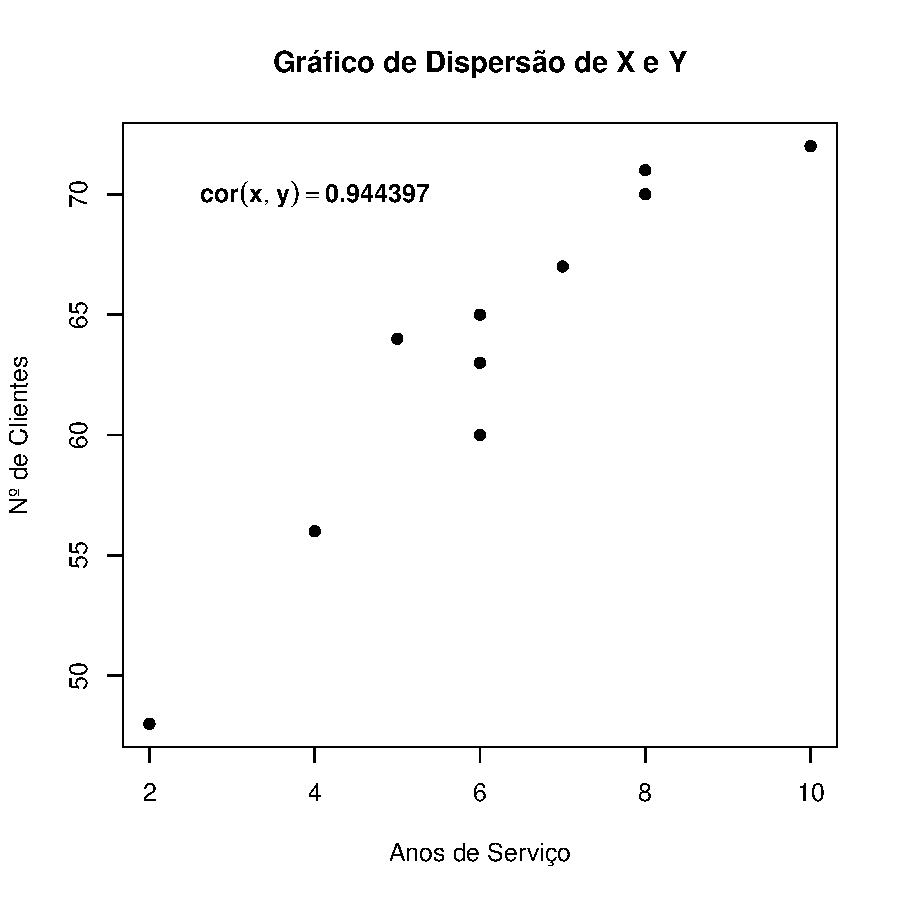
\includegraphics{Aula3-001}
         \end{tabular}  \\
\end{tabular}
\end{frame}

\begin{frame}[fragile]{}
\frametitle{}
\vspace{-0.5cm}
\begin{tabular}{cl}  
        \begin{tabular}{c}
          \parbox{0.5\linewidth}{
          \begin{table}[h!]
  \caption{Renda bruta mensal $(X)$ e porcentagem da renda gasta em saúde $(Y).$}
  \begin{tabular}{ccc}
  \hline
  Família&X&Y\\
  \hline
  A&12&7.2\\
  B&16&7.4\\
  C&18&7.0\\
  D&20&6.5\\
  E&28&6.6\\
  F&30&6.7\\
  G&40&6.0\\
  H&48&5.6\\
  I&50&6.0\\
  J&54&5.5\\
  \hline
  \hline
  \end{tabular}
  \end{table}
          }
        \end{tabular}
           & 
        \begin{tabular}{l}
          \setkeys{Gin}{width=0.4\linewidth}
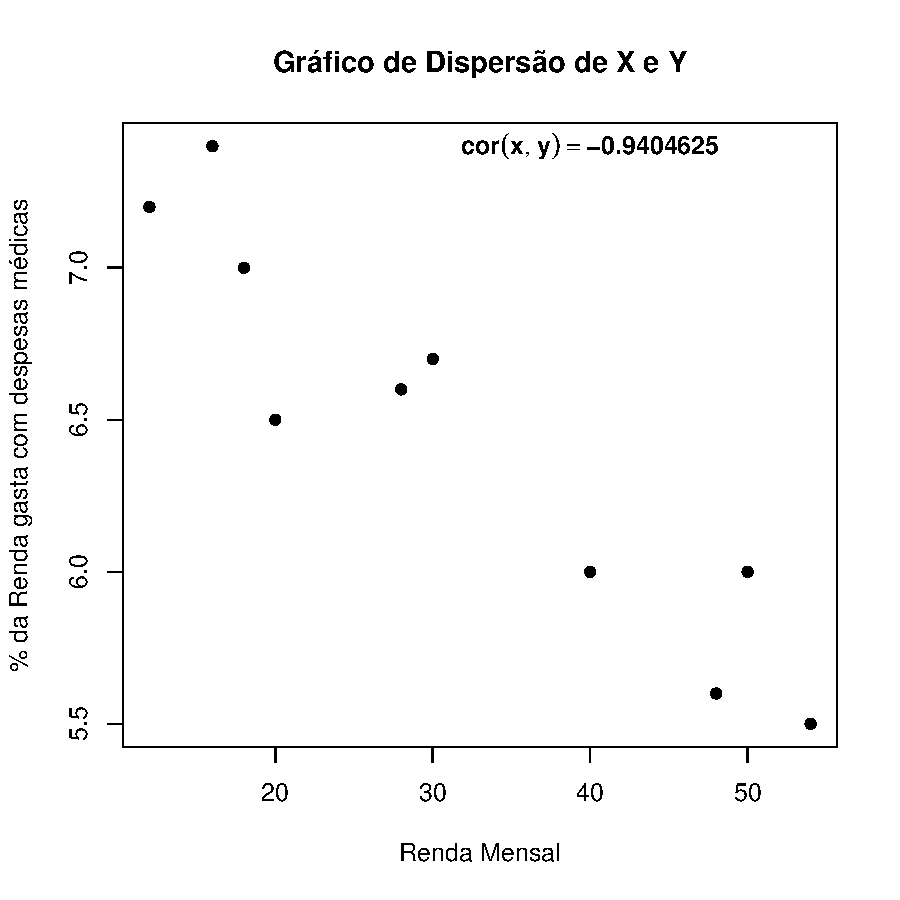
\includegraphics{Aula3-002}
         \end{tabular}  \\
\end{tabular}
\end{frame}

\begin{frame}{}
\frametitle{}
\begin{block}{}
\begin{figure}[H]
    \centering
    \includegraphics[scale=0.5]{figs/correlacao}
    \caption{Representação gráfica de diversos coeficientes de correlação.}
    %\label{figRotulo}
  \end{figure}
\end{block}
\end{frame}

\begin{frame}[fragile]{}
\begin{center}
\setkeys{Gin}{width=0.6\linewidth}
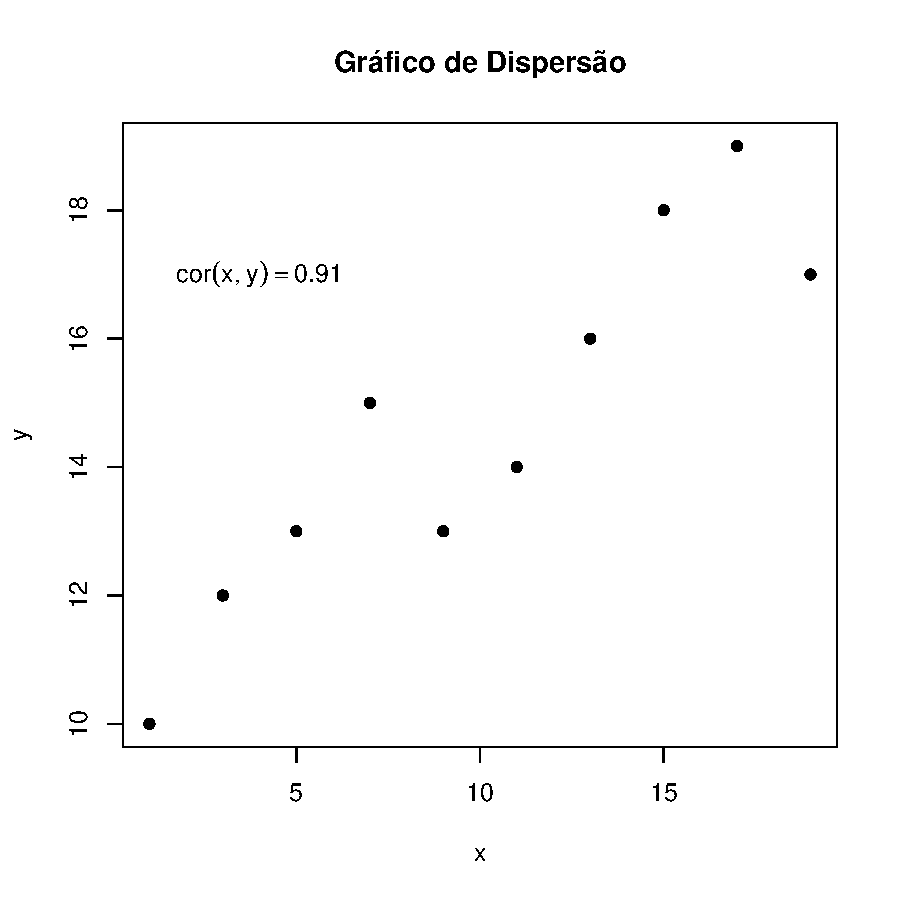
\includegraphics{Aula3-003}
\end{center}
\end{frame}

\begin{frame}[fragile]{}
\begin{center}
\setkeys{Gin}{width=0.6\linewidth}
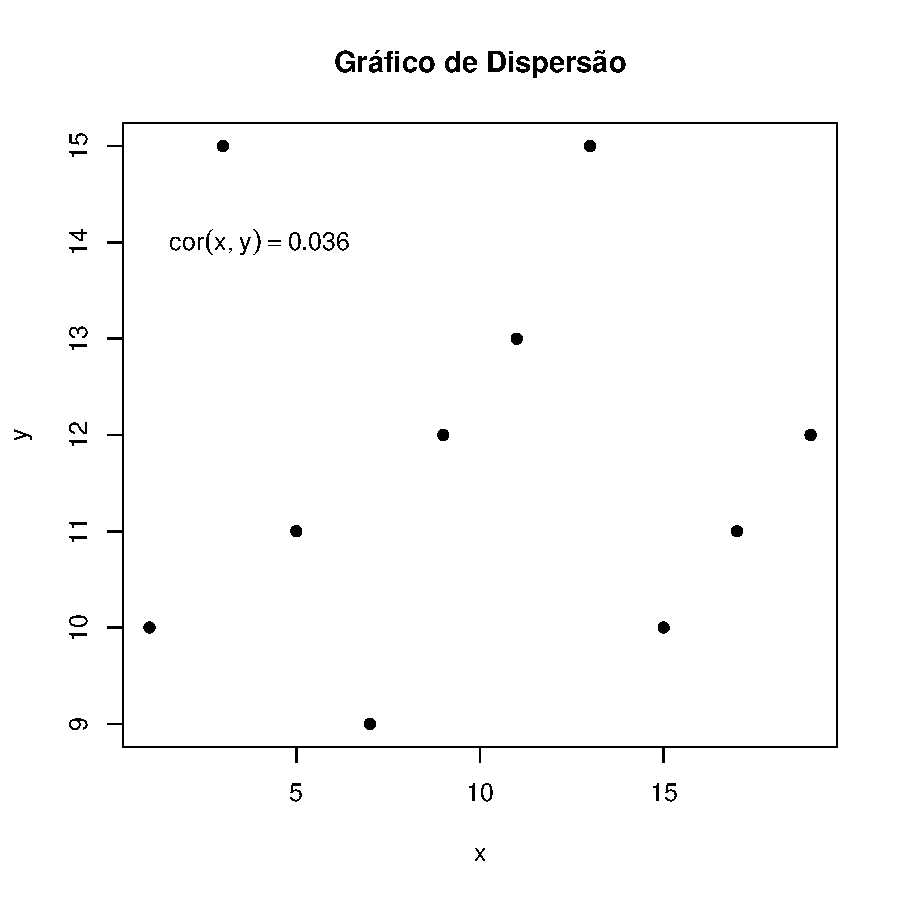
\includegraphics{Aula3-004}
\end{center}
\end{frame}

\begin{frame}[fragile]{}
\begin{center}
\setkeys{Gin}{width=0.6\linewidth}
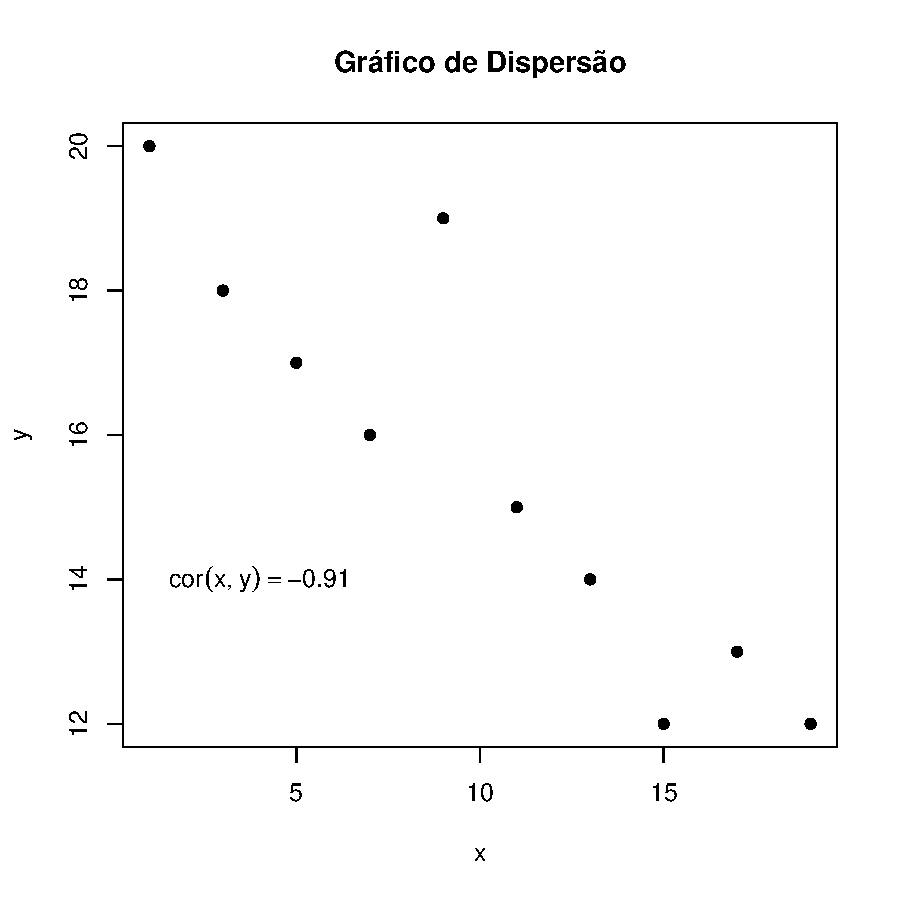
\includegraphics{Aula3-005}
\end{center}
\end{frame}

\begin{frame}[fragile]{}
\begin{center}
\setkeys{Gin}{width=0.6\linewidth}
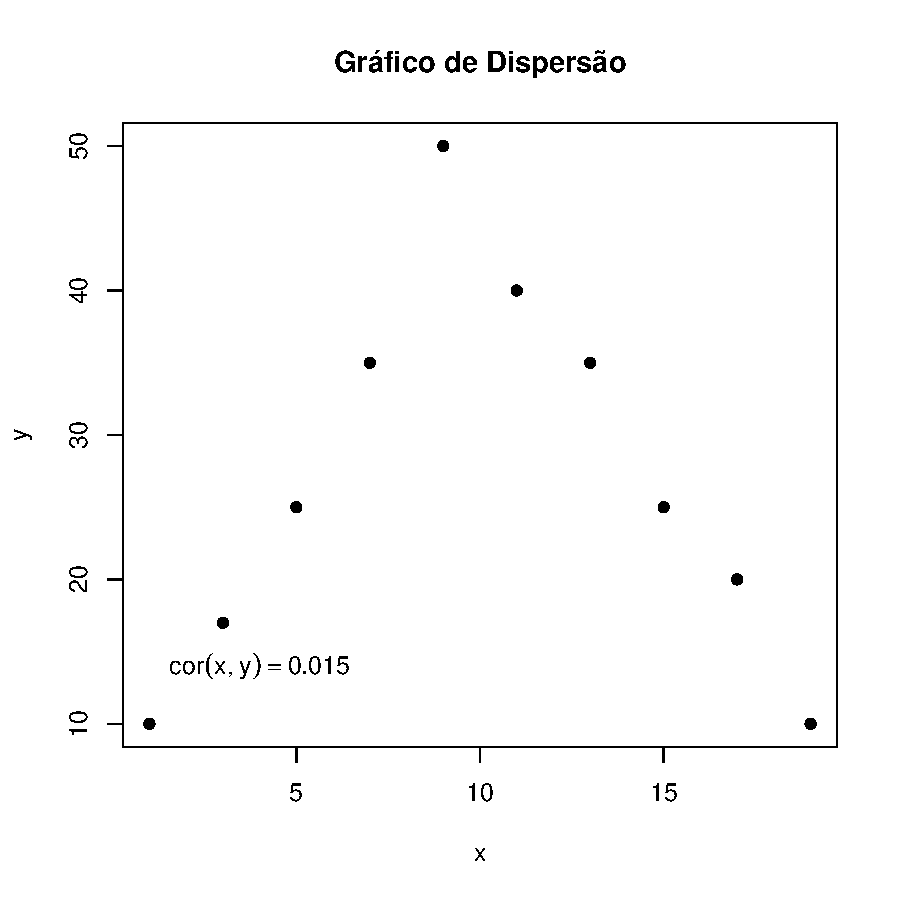
\includegraphics{Aula3-006}
\end{center}
\end{frame}

\begin{frame}{Coeficiente de Correlação Amostral de Pearson}
    \begin{block}{}
    \justifying
    O coeficiente de correlação $(r\ \textrm{ou}\ \hat{\rho})$ mede o grau de associação linear entre duas variáveis aleatórias $X$ e $Y.$ Considere,
    \begin{table}[H]
        \centering
        \begin{tabular}{c|cccc}
             $X_{i}$&$X_{1}$ $X_{2}$ $\cdots$ $X_{n}$ \\
             \hline
             $Y_{i}$&$Y_{1}$ $Y_{2}$ $\cdots$ $Y_{n}$ 
        \end{tabular}
    \end{table}
    Assim, o coeficiente de correlação entre $X$ e $Y$ é dado por:
    
    $$r_{XY}=\dfrac{S_{XY}}{\sqrt{S^{2}_{X}\cdot S_{Y}^{2}}}=
    \dfrac{\dfrac{SPD_{XY}}{n-1}}{\sqrt{\dfrac{SQD_{X}}{n-1}\cdot\dfrac{SQD_{Y}}{n-1}}}= 
    \dfrac{SPD_{XY}}{\sqrt{SQD_{X}\cdot SQD_{Y}}}$$
    
    \end{block}
\end{frame}

\begin{frame}{}
\frametitle{}
%\vspace{-0.6cm}
\begin{block}{}
\justifying
Temos,
$$SPD_{XY}=\sum_{i=1}^{n}X_{i}Y_{i}-\dfrac{\Big({\displaystyle\sum_{i=1}^{n}X_{i}}\Big)\Big({\displaystyle\sum_{i=1}^{n}Y_{i}\Big)}}{n}$$
\pause
$$SQD_{X}=\displaystyle{\sum_{i=1}^{n}X_{i}^{2}}-\dfrac{\Big(\displaystyle{\sum_{i=1}^{n}X_{i}}\Big)^{2}}{n}\quad \textrm{e}\quad SQD_{Y}=\displaystyle{\sum_{i=1}^{n}Y_{i}^{2}}-\dfrac{\Big(\displaystyle{\sum_{i=1}^{n}Y_{i}}\Big)^{2}}{n}$$
\end{block}
\pause
\vspace{-0.06cm}
\begin{block}{}
\justifying
Não é difícil provar que o coeficiente de correlação satisfaz:
$$-1\leq cor(X,Y)\leq 1$$
\end{block}
%\vspace{-0.8cm}
\end{frame}

\begin{frame}{}
    \begin{block}{}
\justifying
{\bf DEF:} Dados $n$ pares de valores $(x_{1}, y_{1}), \cdots, (x_{n}, y_{n}),$ chamaremos de covariância entre as duas variáveis $X$ e $Y$ a igualdade:
$$S_{XY}=cov(X,Y)={\displaystyle \sum_{i=1}^{n}\dfrac{(x_{i}-\bar{x})(y_{i}-\bar{y})}{n}}$$
\end{block}
\pause
\begin{block}{}
\justifying
Com a definição acima, o coeficiente de correlação pode ser escrito como:
$$r_{XY}=cor(X,Y)=\dfrac{cov(X,Y)}{dp(X)dp(Y)}$$
\end{block}
\end{frame}

\begin{frame}{}
\frametitle{}
\begin{block}{}
\justifying
A covariância mede a relação linear entre duas variáveis. A covariância é semelhante à correlação entre duas variáveis, no entanto, elas diferem nas seguintes maneiras:
\end{block}
\pause
\begin{block}{}
\justifying
\begin{itemize}
\item Os coeficientes de correlação são padronizados. Assim, um relacionamento linear perfeito resulta em um coeficiente de correlação 1. A correlação mede tanto a força como a direção da relação linear entre duas variáveis.
\end{itemize}
\end{block}
\pause
\begin{block}{}
\justifying
\begin{itemize}
\item Os valores de covariância não são padronizados. Como os dados não são padronizadas, é difícil determinar a força da relação entre as variáveis.
\end{itemize}
\nocite{roteiro}
\end{block}
\end{frame}

\begin{frame}%[allowframebreaks]
\frametitle{\bf Referências}
%\bibliography{Referencias.bib}
\printbibliography
\end{frame}


\end{document}

%%%%%%%%%%%%%%%%%%%%%%%%%%%%%%%%%%%%%%%%%%%%%%%%%%%%%%%%%%%%%
%%%%%%%%%%%%%%%%%%%%%%%%%%%%%%%%%%%%%%%%%%%%%%%%%%%%%%%%%%%%%
% Partes Retiradas da aula 8
%%%%%%%%%%%%%%%%%%%%%%%%%%%%%%%%%%%%%%%%%%%%%%%%%%%%%%%%%%%%%
%\begin{frame}{}
%\frametitle{}
%\vspace{-0.5cm}
%% Table generated by Excel2LaTeX from sheet 'Plan1'
%\begin{table}[htbp]
%  \centering
%  \caption{Cálculo do coeficiente de correlação.}
%  \resizebox*{0.8\textwidth}{!}{%
%    \begin{tabular}{c|c|c|c|c|c|c|c}
%    \hline
%    Agente & Anos  & Clientes & $x-\bar{x}$ & $y-\bar{y}$ & %$\dfrac{x-\bar{x}}{dp(x)}=z_{x}$ & %$\dfrac{y-\bar{y}}{dp(y)}=z_{y}$ & $z_{x}.z_{y}$ \\
%    \hline
%    A     & 2     & 48    & -3.7  & -8.5  & -1.54 & -1.05 & %1.617 \\
%    B     & 3     & 50    & -2.7  & -6.5  & -1.12 & -0.8  & %0.896 \\
%    C     & 4     & 56    & -1.7  & -0.5  & -0.71 & -0.06 & %0.043 \\
%    D     & 5     & 52    & -0.7  & -4.5  & -0.29 & -0.55 & %0.160 \\
%    E     & 4     & 43    & -1.7  & -13.5 & -0.71 & -1.66 & %1.179 \\
%    F     & 6     & 60    & 0.3   & 3.5   & 0.12  & 0.43  & %0.052 \\
%    G     & 7     & 62    & 1.3   & 5.5   & 0.54  & 0.68  & %0.367 \\
%    H     & 8     & 58    & 2.3   & 1.5   & 0.95  & 0.18  & %0.171 \\
%    I     & 8     & 64    & 2.3   & 7.5   & 0.95  & 0.92  & %0.874 \\
%    J     & 10    & 72    & 4.3   & 15.5  & 1.78  & 1.91  & %3.400 \\
%    \hline
%    Total & 57    & 565   & 0     & 0     &       &       & %8.759 \\
%    \hline
%    \end{tabular}%
%  \label{tab:addlabel}%
%}
%\end{table}%
%$$Cor={\displaystyle %\dfrac{1}{n}\sum_{i=1}^{n}\Biggl(\dfrac{x_{i}-\bar{x}}{dp(X)}\Bi%ggl)\Biggl(\dfrac{y_{i}-\bar{y}}{dp(Y)}\Biggl)}=\dfrac{8.759}{10%}=0.8759$$
%\end{frame}

\section{Medidas Complementares}
\begin{frame}{}
\frametitle{Medidas Complementares para Análise de Dados}
\begin{block}{}
\justifying
\begin{itemize}
\item Extremos: O menor e o maior valor do conjunto de dados;
\item Quartis (Q)
\begin{itemize}
\item $1^{\circ}$ Quartil: deixa um quarto dos valores abaixo, e três quartos acima dele;
\item $2^{\circ}$ Quartil $=$ Mediana: deixa metade dos valores abaixo, e metade acima dele;
\item $3^{\circ}$ Quartil: deixa três quartos dos valores abaixo, e um quarto acima dele;
\end{itemize}
\item Intervalo Interquartil (pode ser considerada uma medida robusta de dispersão).
\end{itemize}
\end{block}
\end{frame}

\begin{frame}{}
\frametitle{Distância Interquartil}
\begin{block}{}
\justifying
Uma medida de dispersão alternativa ao desvio padrão é a distância interquartil, definida como a diferença entre o terceiro e primeiro quartis, ou seja:
$$d_{q}=q_{3}-q_{1}$$
\end{block}
\end{frame}

%\begin{frame}{}
%\frametitle{Cálculo dos Quartis}
%\begin{block}{}
%\justifying
%Seja $n$ o número total de elementos da amostra e %calcule $\dfrac{j(n+1)}{4},$ para $j=1,2$ e $3$. %Desta forma $q_{j}$ será um elemento entre %$X_{k}$ e $X_{k+1},$ onde $k$ é o maior inteiro %menor ou igual a 
%$\dfrac{j(n+1)}{4}$ e será calculado da seguinte %forma:
%\begin{equation}
%q_{j}=X_{(k)}+\Biggl(\dfrac{j(n+1)}{4}-k\Biggl%)(X_{(k+1)}-X_{(k)})
%\end{equation}
%
%Podemos observar que quando $k$ é um valor %inteiro, o quantil será o próprio $X_{(k)}$, isto %é, $q_{j}=X_{(k)}$, onde 
%$k=\dfrac{j(n+1)}{4}, j=1,2,3$.
%
%\end{block}
%\end{frame}

\begin{frame}{}
\frametitle{}
\begin{block}{}
\justifying
Os cinco valores, $x_{(1)}, q_{1}, q_{2}, q_{3}\ e\ x_{(n)}$ são importantes para se ter uma boa ideia da assimetria da distribuição dos dados. Para uma distribuição simétrica 
ou aproximadamente simétrica, deveríamos ter:
\begin{enumerate}
\item[(a)] $q_{2}-x_{(1)}\approx x_{(n)}-q_{2};$
\item[(b)] $q_{2}-q_{(1)}\approx q_{(3)}-q_{2};$
\item[(c)] $q_{1}-x_{(1)}\approx x_{(n)}-q_{3};$
\item[(d)] distâncias entre mediana e $q_{1}, q_{3}$ menores do que distâncias entre os extremos e $q_{1}, q_{3}.$
\end{enumerate}
\end{block}
\end{frame}

\begin{frame}{}
\frametitle{}
\begin{block}{}
\justifying
A diferença $q_{2}- x_{(1)}$ é chamada dispersão inferior e $x_{(n)}-q_{2}$ é a dispersão superior.
A condição (a) nos diz que estas duas dispersões devem ser aproximadamente iguais, para uma distribuição 
aproximadamente simétrica. A próxima Figura ilustra estes fatos para a chamada distribuição normal ou gaussiana.
\end{block}
\end{frame}

\begin{frame}{}
\frametitle{}
\begin{block}{}
\justifying
\begin{figure}[H]
    \centering
    \begin{tikzpicture}[scale=0.5]
%\node {\includegraphics{Fig7.jpg}};
\draw[line width=2] (-12.9,-4.2)--(13.4,-4.2);
\draw[line width=2] (-9.2,-4)--(-9.2,-4.4);
\draw[line width=2] (9.1,-4)--(9.1,-4.4);
\draw[line width=2] (0,-4)--(0,-4.4);
\draw[line width=2] (-2.7,2.7)--(-2.7,-4.4);
\draw[line width=2] (2.6,3)--(2.7,-4.4);
\draw[line width=4] (-11.3,-3.9) .. controls (-6.6,-3.6) and (-5,-2) .. (-3.2,1.7) .. 
controls (-2.2,4.2) and (-0.7,5.5) .. (1.1,4.6) .. 
controls (3.4,3) and (4.2,-1.4) .. (6.9,-2.9) .. 
controls (8.2,-3.6) and (9.9,-3.8) .. (11.8,-3.9);
\draw[line width=3, fill=Lightblue] (-2.7,2.7) .. controls (-0.6,6.5) and (1.6,4.6) .. (2.6,3) .. 
controls (2.6,1.3) and (2.7,-1.5) .. (2.7,-4.2) .. 
controls (1,-4.2) and (-1.4,-4.2) .. (-2.7,-4.2) .. 
controls (-2.7,-1.9) and (-2.7,0.3) .. (-2.7,2.7);
\node at (-0.1,0.1) {\small{{\bf $50\%$ das}}};
\node at (-0.1,-0.7) {\small{{\bf observações}}};
\node at (-9.2,-5) {{$x_{(1)}$}};
\node at (-2.7,-5) {{$q_{1}$}};
\node at (0,-5) {{$q_{2}$}};
\node at (2.7,-5) {{$q_{3}$}};
\node at (9.2,-5) {{$x_{(n)}$}};
\end{tikzpicture}
    \caption{Uma distribuição simétrica: normal ou gaussiana \cite{Morettin09}.}
    \label{Fig7_ex}
  \end{figure}
\end{block}
\end{frame}

\begin{frame}{}
\frametitle{}
\begin{block}{}
\justifying
As cinco estatísticas de ordem consideradas acima podem ser representadas esquematicamente como na próxima Figura, onde também incorporamos o número de 
observações, $n.$ Representamos a mediana por $md,$ os quartis por $q$ e os extremos por $E.$
\begin{figure}[H]
    \centering
    \begin{tikzpicture}[scale=0.5]
%\node {\includegraphics{Fig8.jpg}};
\draw[line width=2](-4.6,-2.9)--(-4.6,2.5) -- 
(5.9,2.5) -- (5.9,-2.9);
\node at (-5.4,1.8) {md};
\node at (-5.4,-0.1) {$q$};
\node at (-5.4,-1.9) {E};
\node at (-4,-0.1) {$q_{1}$};
\node at (-3.8,-1.9) {$x_{(1)}$};
\node at (0.6,3) {$n$};
\node at (0.6,2) {$q_{2}$};
\node at (4.9,-0.1) {$q_{3}$};
\node at (4.9,-1.9) {$x_{(n)}$};
\end{tikzpicture}
    \caption{Esquema dos cinco números (\cite{Morettin09}).}
    \label{Fig8_ex}
  \end{figure}
\end{block}
\end{frame}

% \begin{frame}{}
% \frametitle{}
% \begin{block}{}
% \begin{figure}
% \centering
% \begin{tikzpicture}[xscale=1.5, yscale=7, declare function={stdnorm(\x) = 1/(sqrt(2*pi))*exp(-0.5*(pow(\x,2)));}]
% \fill[gray] (-2.5,0) -- plot [domain=-2.5:-3/2, samples=50] (\x, {stdnorm(\x)}) -- (-3/2,0) -- cycle;
% \fill[gray] (3/2,0) -- plot [domain=3/2:5/2, samples=50] (\x, {stdnorm(\x)}) -- (5/2,0) -- cycle;
% \draw [thick, domain=-2.5:2.5, samples=50] plot (\x, {stdnorm(\x)});
% \draw [->] (-3,0) -- (3,0) ;
% \node [below right] at (3,0) {$z$} ;
% \draw [dashed] (0,0) -- (0,{stdnorm(0)}) ;
% \draw [dashed] (-3/2,0) -- (-3/2,{stdnorm(-3/2)}) ;
% \draw [dashed] (3/2,0) -- (3/2,{stdnorm(3/2)}) ;
% \node [below] at (0,0) {$0$};
% \node [below] at (-3/2,0) {$-1.96$};
% \node [below] at (3/2,0) {$1.96$};
% \node [above] at (-2.5,0.1) {\small{RR$\Ho$}};
% \node [above] at (2.5,0.1) {\small{RR$\Ho$}};
% \node [above] at (-1,0.5) {\small{RNR$\Ho$}};
% \node [above] at (2,0.5) {$z_{cal}=3.25$};
% \node [above] at (2,0.4) {p-valor$=0.0012$};
% \node [above] at (2,0.3) {$\alpha=0.05$};
% %\draw[->] (-2.7,0.15) .. controls (.-2,.2) .. (-1.9, 0.03);
% \draw[->] (-2.2,0.15) to [out=20,in=90] (-1.9,0.02);
% \draw[->] (2.2,0.15) to [out=160,in=90] (1.9,0.02);
% \draw[->] (-0.6,0.55) to [out=0,in=90] (0.1,0.3);
% %\draw [->,thick] (2.7,0.15) to [out=120,in=0] (2.3,0.3)
% %to [out=0,in=90] (1.9,0.03);
% %\draw (0,0) .. controls (0,4) and (4,0) .. (4,4)
% %\draw[->] ( 3,0.15) .. controls (. 30,.2) .. (1.9, 0.03);
% %\node at (1.8,{stdnorm(2.3)}) {\small{$\alpha/2$}};
% %\node at (-1.8,{stdnorm(2.3)}){\small{$\alpha/2$}};
% \end{tikzpicture}
% %\caption{Região crítica para $\Ho: \mu = 50$ versus $\Hi: \mu \neq 50$ e $n = 25$}
% \end{figure}
% \end{block}
% \end{frame}

\section{Box Plot}
\begin{frame}{}
\frametitle{Box Plot}
\begin{block}{}
\justifying
O boxplot (gráfico de caixa) é um gráfico utilizado para avaliar a distribuição empírica do dados. O boxplot é formado pelo primeiro e terceiro quartil e pela mediana. Para construir este diagrama, consideremos um retângulo onde estão representados a mediana e os quartis. A partir do retângulo, para cima, segue uma linha até o ponto mais remoto que não exceda $LS = q_{3} + (1,5)d_{q},$ chamado limite superior. De modo similar, da parte inferior do retângulo, para baixo, segue uma linha até o ponto mais remoto que não seja menor do que 
$LI = q_{1}-(1,5)d_{q},$ chamado limite inferior.
\end{block}
\end{frame}

\begin{frame}{}
\frametitle{Box-Plot}
\begin{block}{}
\justifying
Os valores compreendidos entre esses dois limites são chamados valores adjacentes. As observações que estiverem acima do limite superior ou abaixo do limite inferior estabelecidos serão chamadas pontos exteriores e representadas por asteriscos. Essas são observações destoantes das demais e
podem ou não ser o que chamamos de outliers ou valores atípicos.
\end{block}
\end{frame}

\begin{frame}{}
\frametitle{Box-Plot}
\begin{block}{}
\justifying
\begin{figure}[H]
\centering
\caption{Esquema de um BoxPlot \cite{Morettin09}.}
\begin{tikzpicture}[scale=0.4]
%\node {\includegraphics{Fig9.jpg}};
\draw[line width=2] (-5.2,7) -- (-5.2,-7);
\draw[line width=2] (4.7,7) -- (4.7,-7);
\draw[line width=2, dashed] (-5.2,6.8) -- (5.2,6.8);
\draw[line width=2, dashed] (-5,-6.8) -- (5,-6.8);
\draw[line width=2] (-5.4, 1.7) -- (-4.9,1.7);
\draw[line width=2] (-5.4,-0.5) -- (-4.9,-0.5);
\draw[line width=2] (-5.4,-1.7) -- (-4.9,-1.7);
\draw[line width=2] (4.5,6.8) -- (6.5,6.8);
\draw[line width=2] (4.7,-6.8) -- (6.5,-6.8);
\draw[line width=1, ->] (5.7,5) -- (5.7,6.7);
\node at (5.7,3.9) {$ {\scriptstyle \frac{3}{2}d_{q}}$};
\draw[line width=1, ->] (5.7,3) -- (5.7,1.9);
\draw[line width=2] (4.7,1.7) -- (6.3,1.7);
\draw[line width=1, ->] (5.7,0.7) -- (5.7,1.5);
\node at (5.7,0.2) {$ {\scriptstyle d_{q}}$};
\draw[line width=1, ->] (5.7,-0.3) -- (5.7,-1.4);
\draw[line width=2] (4.7,-1.7) -- (6.3,-1.7);
\draw[line width=1, ->] (5.7,-3) -- (5.7,-1.9);
\node at (5.7,-3.8) {$ {\scriptstyle \frac{3}{2}d_{q}}$};
\draw[line width=1, ->] (5.7,-4.7) -- (5.7,-6.5);
\node at (-6,1.6) {$q_{3}$};
\node at (-6,-0.6) {$q_{2}$};
\node at (-6,-1.6) {$q_{1}$};
\draw[line width=2] (-0.9,6.1) -- (-0.2,6.1);
\draw[line width=2] (-0.6,6.1) -- (-0.6,1.7) -- 
(0.7,1.7) -- (0.7,-1.7) -- (-1.7,-1.7) -- (-1.7,1.7) --
(-0.6,1.7);
\draw[line width=2] (-1.7,-0.6) -- (0.7,-0.6);
\draw[line width=2] (-0.6,-1.7) -- (-0.6,-5.6);
\draw[line width=2] (-0.9,-5.6) -- (-0.2,-5.6);
\node at (-0.6,7.2) {$*$};
\node at (-0.6,-7.2) {$*$};
\end{tikzpicture}
\label{Fig9_ex}
\end{figure}
\end{block}
\end{frame}

\begin{frame}{}
\frametitle{}
\begin{block}{}
\justifying
O box plot dá uma idéia da posição, dispersão, assimetria, caudas e dados discrepantes.
A posição central é dada pela mediana e a dispersão por $d_{q}.$ As posições relativas de $q_{1}, q_{2}, q_{3}$
dão uma noção da assimetria da distribuição. Os comprimentos das caudas são dados pelas
linhas que vão do retângulo aos valores remotos e pelos valores atípicos. Veja esse  
\href{https://www.geogebra.org/m/aurvf6dz}{exemplo.}
\end{block}
\end{frame}

\section{Assimetrias e Transformações}
\begin{frame}{}
\frametitle{Assimetrias}
\begin{block}{}
\begin{minipage}{0.4\textwidth}
\begin{figure}[h]
\centering
\caption{Distribuições assimétricas \cite{Morettin09}.}
\begin{tikzpicture}[scale=0.5]
%\node {\includegraphics{Fig10.jpg}};
\draw[line width=2, red] (-14.8,-1.7) .. 
controls (-13.4,-1.3) and (-12.6,2.2) .. (-11,2.2) .. 
controls (-9.4,1.8) and (-8,-0.2) .. (-5.7,-0.9) .. 
controls (-5,-1.2) and (-3.9,-1.5) .. (-2.1,-1.6);
\draw[line width=2, red] (-15.1,-2) -- (-1.9,-2);
\node at (-9.8,-2.7) {Assimétrica à direita};
\end{tikzpicture}
\label{Fig10_ex}
\end{figure}
\end{minipage}\hfill
\begin{minipage}{0.5\textwidth}
\begin{figure}[h]
\centering
\caption{Distribuições assimétricas \cite{Morettin09}.}
\begin{tikzpicture}[scale=0.4]
%\node {\includegraphics{Fig10.jpg}};
\draw[line width=2, red] (1.1,-1.8) .. controls (5.3,-1.6) and (6.9,1.2) .. (8.5,2.4) .. controls (9.6,3.1) and (9.9,2.6) .. (10.4,2) .. controls (11.2,1) and (12.5,-1.5) .. (15,-1.8);
\draw[line width=2, red] (1,-2.3) -- (15.2,-2.3);
\node at (7.8,-3.2) {Assimétrica à esquerda};
\end{tikzpicture}
\label{Fig10_ex}
\end{figure}
\end{minipage}
\end{block}
\end{frame}

\begin{frame}{}
\frametitle{Transformações}
\begin{block}{}
\justifying
Vários procedimentos estatísticos são baseados na suposição de que os dados provêm
de uma distribuição normal (em forma de sino) ou então mais ou menos simétrica.
Mas, em muitas situações de interesse prático, a distribuição dos dados da amostra
é assimétrica e pode conter valores atípicos, como vimos em exemplos anteriores.
\end{block}
\end{frame}

\begin{frame}{}
\frametitle{}
\begin{block}{}
\justifying
Se quisermos utilizar tais procedimentos, o que se propõe é efetuar uma transformação
das observações, de modo a se obter uma distribuição mais simétrica e próxima
da normal. Uma família de transformações frequentemente utilizada é
\[
X^{*}=\left\{
\setlength\arraycolsep{0pt}
\begin{array}{lr}
X^{p},                              &\quad \textrm{se}\quad p>0\\
&\\
\ln{(X)},                           &\quad \textrm{se}\quad p=0\\
&\\
-X^{p},                             &\quad \textrm{se}\quad p<0\\
\end{array}
\right.
\]
Normalmente, o que se faz é experimentar valores de $p$ na sequência 
$\cdots, -3, -2, -1, -1/2, -1/3, -1/4, 0, 1/4, 1/3, 1/2, 1, 2, 3,\cdots$
\end{block}
\end{frame}

\begin{frame}{}
\frametitle{}
\begin{block}{}
\justifying
Para cada valor de $p$ obtemos gráficos apropriados (histogramas, desenhos esquemáticos etc.)
para os dados originais e transformados, de modo a escolhermos o valor mais adequado de p. Para dados positivos, 
a distribuição dos dados é usualmente assimétrica à direita. Para essas distribuições, a transformação acima com 
$0 < p < 1$ é apropriada, pois valores grandes de $x$ decrescem mais, relativamente a valores pequenos. Para distribuições assimétricas à esquerda, tome $p > 1.$
\end{block}
\end{frame}

\begin{frame}[allowframebreaks]
\frametitle{\bf Referências}
\printbibliography
\end{frame}


%\begin{frame}{}
%\frametitle{}
%\begin{figure}[H]
%    \centering
%    \includegraphics[height=0.4\textwidth%,width=15cm]{figs/Fig11}
%    \caption{Exemplo de Histogramas para %dados transformados (\cite{Morettin09}).}
%    \label{Fig101_ex}
%  \end{figure}
%\end{frame}